\documentclass[a4paper, 14pt]{extarticle}

% Поля
%----------------------
\usepackage{geometry}
\geometry{a4paper,left=2cm,right=1cm,
    top=2cm,bottom=2cm,bindingoffset=0cm}
%----------------------

% Russian-specific packages
%----------------------
\usepackage[T2A]{fontenc}
\usepackage[utf8]{inputenc}
\usepackage[english, main=russian]{babel}
%----------------------

\usepackage{textcomp}

% Красная строка
%----------------------
\usepackage{indentfirst}
%----------------------

% Graphics
%----------------------
\usepackage{graphicx}
\graphicspath{ {./images} }
\usepackage{wrapfig}
%----------------------

% Import minted
%----------------------
\usepackage{minted}
%----------------------

% Tables

%----------------------
\usepackage{longtable}
\usepackage{ragged2e}
\usepackage{booktabs}
\usepackage{array}
\usepackage{caption}
\usepackage{float}

%----------------------

\linespread{1.3}
\sloppy
\clubpenalty=10000
\widowpenalty=10000

\begin{document}

%--------------------------------------
%			ТИТУЛЬНЫЙ ЛИСТ
%--------------------------------------
\begin{titlepage}
\thispagestyle{empty}
\newpage


%Шапка титульного листа
%--------------------------------------
\vspace*{-60pt}
\hspace{-65pt}
\begin{minipage}{0.3\textwidth}
\hspace*{-20pt}\centering

\includegraphics[width=\textwidth]{emblem}
\end{minipage}
\begin{minipage}{0.67\textwidth}\small \textbf{
\vspace*{-0.7ex}
\hspace*{-6pt}\centerline{Министерство науки и высшего образования Российской Федерации}
\vspace*{-0.7ex}
\centerline{Федеральное государственное бюджетное образовательное учреждение }
\vspace*{-0.7ex}
\centerline{высшего образования}
\vspace*{-0.7ex}
\centerline{<<Московский государственный технический университет}
\vspace*{-0.7ex}
\centerline{имени Н.Э. Баумана}
\vspace*{-0.7ex}
\centerline{(национальный исследовательский университет)>>}
\vspace*{-0.7ex}
\centerline{(МГТУ им. Н.Э. Баумана)}}
\end{minipage}
%--------------------------------------

%Полосы
%--------------------------------------
\vspace{-25pt}
\hspace{-35pt}\rule{\textwidth}{2.3pt}

\vspace*{-20.3pt}
\hspace{-35pt}\rule{\textwidth}{0.4pt}
%--------------------------------------

\vspace{1.5ex}
\hspace{-35pt} \noindent \small ФАКУЛЬТЕТ\hspace{80pt} <<Информатика и системы управления>>

\vspace*{-16pt}
\hspace{47pt}\rule{0.83\textwidth}{0.4pt}

\vspace{0.5ex}
\hspace{-35pt} \noindent \small КАФЕДРА\hspace{50pt} <<Теоретическая информатика и компьютерные технологии>>

\vspace*{-16pt}
\hspace{30pt}\rule{0.866\textwidth}{0.4pt}
  
\vspace{11em}

\begin{center}
\Large {\bf Лабораторная работа №4} \\ 
\large {\bf по курсу <<Базы данных>>} \\

% Labname
\large <<Преобразование модели семантических объектов в реляционную модель>> \\
\end{center}\normalsize

\vspace{8em}


\begin{flushright}
  {Студент группы ИУ9-51Б Киселев К.А. \hspace*{15pt}\\ 
  \vspace{2ex}
  Преподаватель Вишняков И.Э. \hspace*{15pt}}
\end{flushright}

\bigskip

\vfill
 

\begin{center}
\textsl{Москва 2023}
\end{center}
\end{titlepage}
%--------------------------------------
%		КОНЕЦ ТИТУЛЬНОГО ЛИСТА
%--------------------------------------

\newpage




\section{Постановка задачи}

\begin{enumerate}
	\item{Преобразовать модель семантических объектов, созданную в лабораторной работе №2, в реляционную модель согласно процедуре преобразования.}
	\item{Сопоставить результаты проектирования с использованием модели «сущность-связь» и модели семантических объектов (лабораторные работы №№3,4).}
	\item{Обосновать различия результатов, выявить и исправить ошибки проектирования.}
\end{enumerate}

\newpage

\section{Практическая реализация}

В соответствии с правилами преобразования, из созданной ранее модели семантических объектов, представленной на рисунке \ref{fig:som_model}, получили реляционную модель, изображенную на  рисунке \ref{fig:relation_model_lab4}.

\begin{figure}[H]
\centering
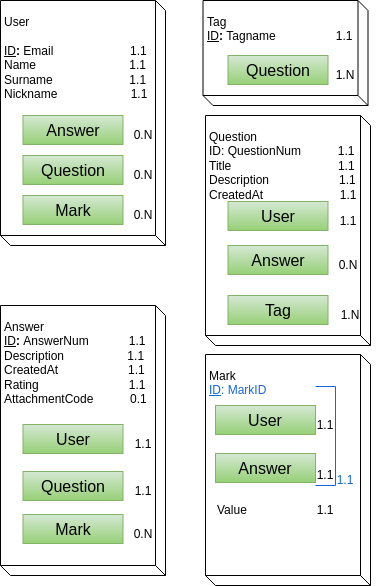
\includegraphics[width=0.4\textwidth]{Diagram3} 
\caption{Модель семантических объектов} 
\label{fig:som_model}
\end{figure}


\begin{figure}[ht]
\centering
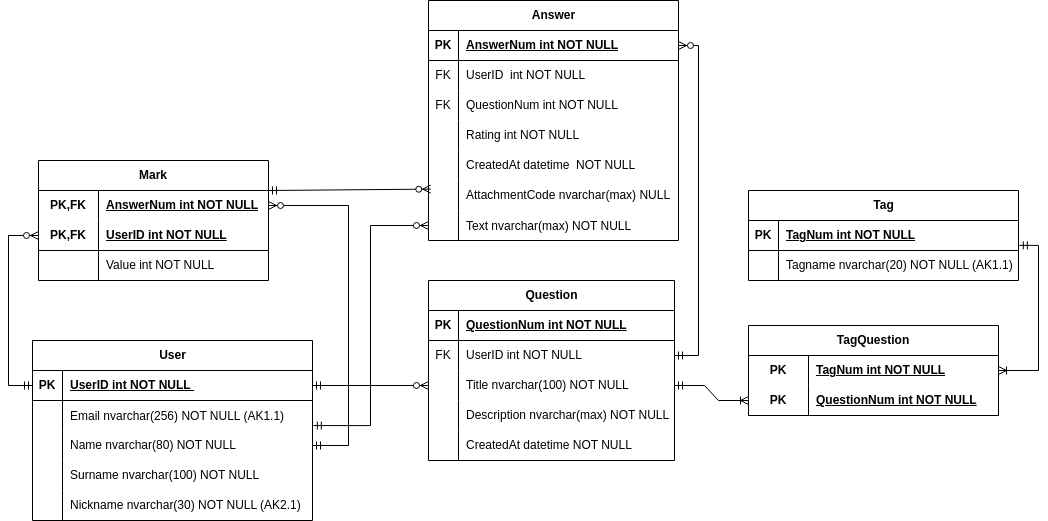
\includegraphics[width=0.6\textwidth]{Diagram1}
\caption{Реляционная модель, полученная из модели семантических объектов.} 
\label{fig:relation_model_lab4}
\end{figure}

На рисунке \ref{fig:relation_model_lab3} представлена полученная на лабораторной работе №3 реляционная модель.

\begin{figure}[ht]
\centering
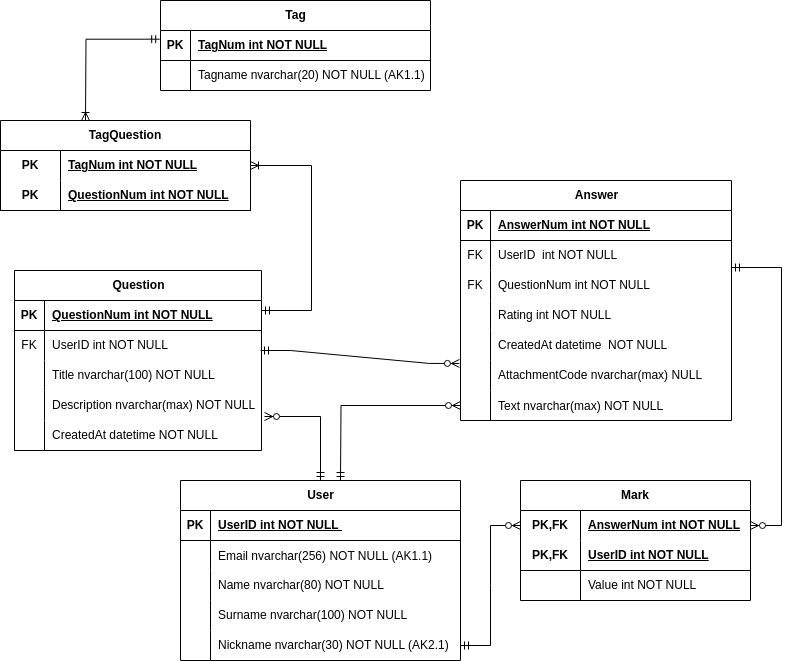
\includegraphics[width=0.6\textwidth]{Diagram2}
\caption{Реляционная модель, полученная из модели "сущность-связь".} 
\label{fig:relation_model_lab3}
\end{figure}


Обе реляционные модели на рисунках \ref{fig:relation_model_lab4}–\ref{fig:relation_model_lab3} описывают одну и ту же предметную область. При сравнении результатов проектирования реляционных моделей, полученных из модели «сущность-связь» и модели семантических объектов, различий не было выявлено.

\end{document}
